\section{Cơ sở lý thuyết}


\subsection{Giới thiệu Machine Learning}

\indent Học máy (machine learning) là một lĩnh vực của trí tuệ nhân tạo liên quan đến việc nghiên cứu và xây dựng các kĩ thuật cho phép các hệ thống "học" tự động từ dữ liệu để giải quyết những vấn đề cụ thể. Lịch sử học máy bắt đầu từ những năm 1950 với các nỗ lực đầu tiên để mô phỏng khả năng học của con người thông qua máy tính. Tuy nhiên, cho đến đầu thập kỷ 21, học máy mới trở nên phổ biến và mạnh mẽ nhờ vào sự tiến bộ của phần cứng và khả năng tính toán.

\indent Trong thập kỷ gần đây, sự phát triển của các thuật toán học máy, kết hợp với dữ liệu lớn và sức mạnh tính toán ngày càng tăng, đã đưa học máy vào tầm tay của nhiều người và ứng dụng rộng rãi trong nhiều lĩnh vực, bao gồm nhận dạng hình ảnh, ngôn ngữ tự nhiên và IoT (Internet of Things).

\subsection{Giới thiệu mô hình LSTM}

\subsubsection{Giới thiệu tổng quan}

\indent Mạng bộ nhớ dài - ngắn (Long Short Term Memory networks), thường được gọi là LSTM - là một dạng đặc biệt của RNN, nó có khả năng học được các phụ thuộc xa. LSTM được giới thiệu bởi Hochreiter \& Schmidhuber vào năm 1997, và sau đó đã được cải tiến và phổ biến bởi rất nhiều người trong ngành. Chúng hoạt động cực kì hiệu quả trên nhiều bài toán khác nhau nên dần đã trở nên phổ biến như hiện nay.

\indent LSTM được thiết kế để tránh được vấn đề phụ thuộc xa (long-term dependency). Việc nhớ thông tin trong suốt thời gian dài là đặc tính mặc định của chúng, chứ ta không cần phải huấn luyện nó để có thể nhớ được. Tức là ngay nội tại của nó đã có thể ghi nhớ được mà không cần bất kì can thiệp nào.

\indent Mọi mạng hồi quy đều có dạng là một chuỗi các mô-đun lặp đi lặp lại của mạng nơ-ron. Với mạng RNN chuẩn, các mô-dun này có cấu trúc rất đơn giản, thường là một tầng tanh. LSTM cũng có kiến trúc dạng chuỗi như vậy, nhưng các mô-đun trong nó có cấu trúc khác với mạng RNN chuẩn. Thay vì chỉ có một tầng mạng nơ-ron, chúng có tới 4 tầng tương tác với nhau một cách rất đặc biệt.

\begin{figure}[H]
    \centering
    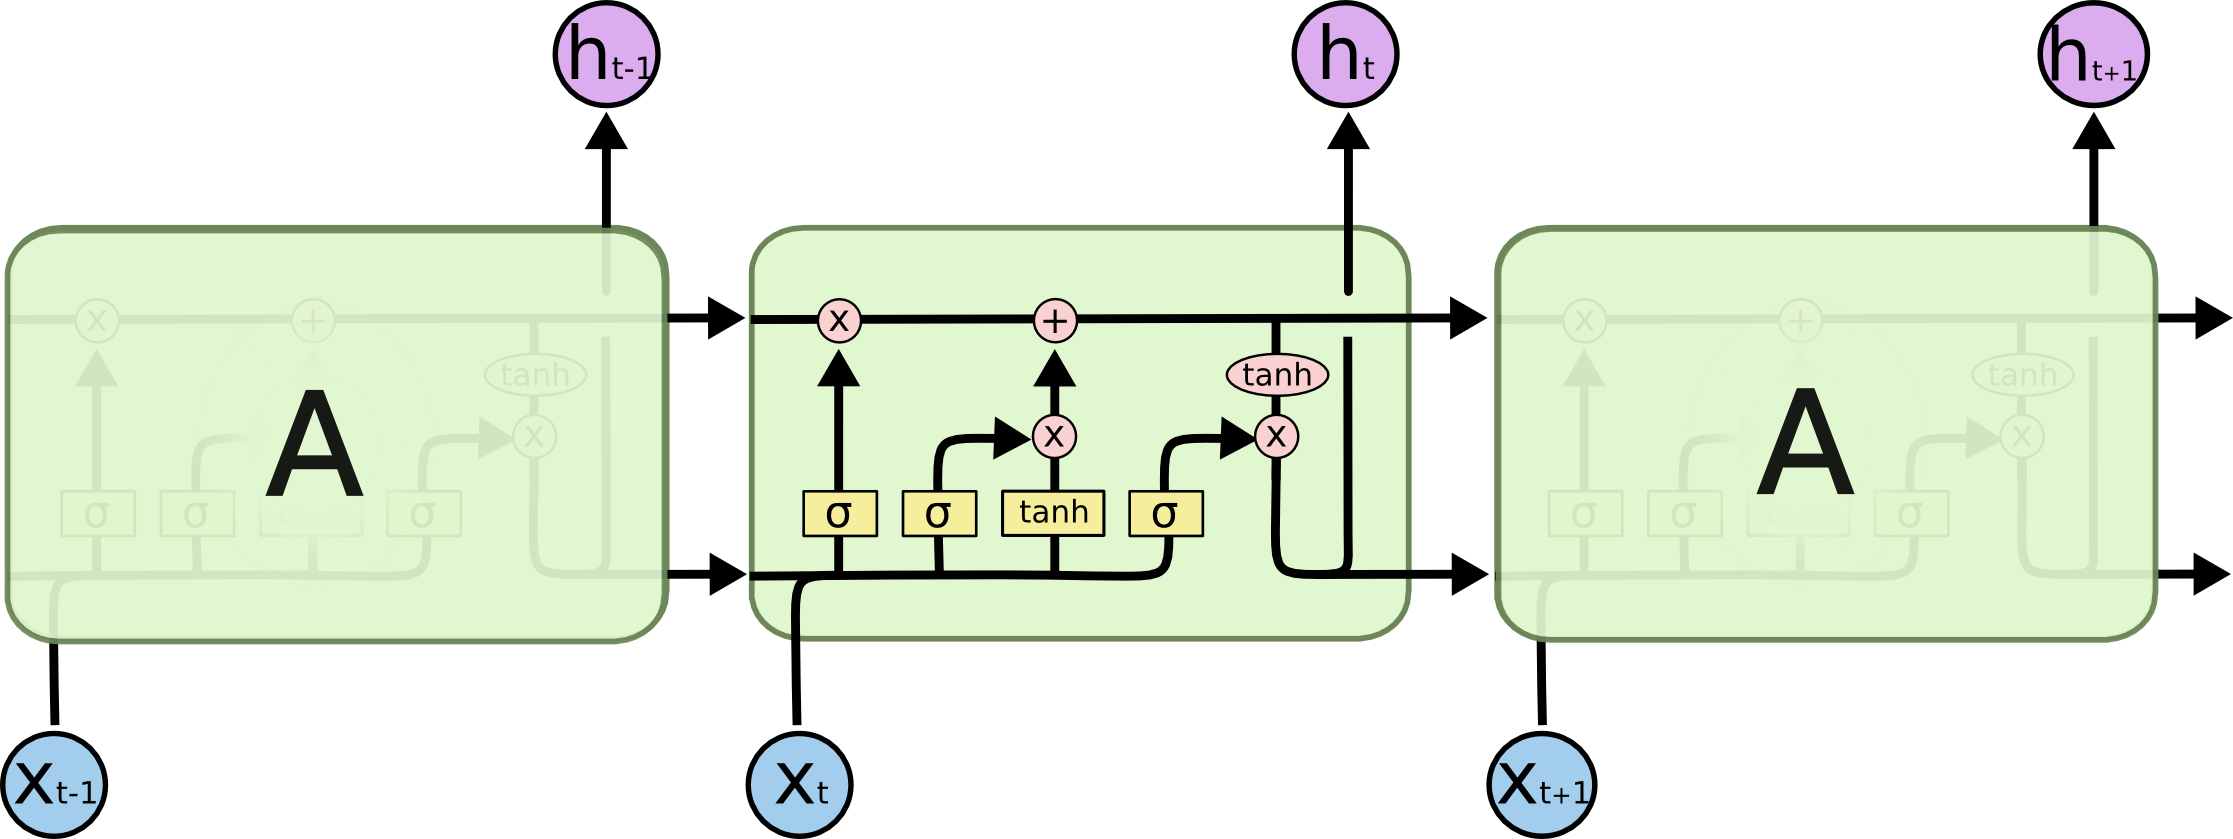
\includegraphics[width=14cm]{Images/Theoretical basis/LSTM.png}
\caption{Mô hình LSTM với 4 lớp tương tác}
\end{figure}

\subsubsection{Ưu và nhược điểm của mô hình LSTM}

\begin{enumerate}[-]
    \item Ưu điểm
    \begin{itemize}
        \item LSTM được thiết kế để xử lý dữ liệu chuỗi và giữ thông tin từ quá khứ, giúp nó phù hợp cho nhiều loại dự đoán chuỗi như ngôn ngữ tự nhiên, dự đoán chuỗi thời gian, v.v.
        \item LSTM có khả năng học và giữ lại thông tin lâu dài, giúp chúng phát hiện và theo dõi các mối quan hệ phức tạp trong dữ liệu dài hạn.
        \item LSTM sử dụng cổng quên (forget gate) để kiểm soát việc giữ và quên thông tin, giúp giảm hiện tượng triệt tiêu gradient, vấn đề thường gặp trong các mô hình RNN.
        \item Có thể kết hợp nhiều lớp LSTM để tạo thành các mô hình học sâu phức tạp hơn, linh hoạt trong việc xử lý nhiều loại dữ liệu và nhiều mức độ phức tạp.
    \end{itemize}
    \item  Nhược điểm
    \begin{itemize}
        \item Mô hình LSTM có khả năng tính toán khá phức tạp, đặc biệt khi được sử dụng trong các mô hình lớn với nhiều tham số.
        \item Do tính toán phức tạp, việc huấn luyện mô hình LSTM có thể mất nhiều thời gian, đặc biệt là khi làm việc với dữ liệu lớn.
        \item Mô hình LSTM có nguy cơ cao về overfitting, đặc biệt khi kích thước dữ liệu huấn luyện ít và mô hình quá phức tạp.
        \item Mặc dù LSTM giảm vấn đề triệt tiêu gradient, nhưng không giải quyết hoàn toàn vấn đề gradient exploding.
    \end{itemize}
\end{enumerate}


\subsection{Giới thiệu thiết bị sử dụng}

\subsubsection{Flex sensors}

\subsubsubsection{Tổng quan} 

\indent Cảm biến uốn cong (flex sensor) thực chất là một biến trở có khả năng thay đổi điện trở khi được uốn cong. Vì điện trở biến thiên tỷ lệ thuận trực tiếp với độ uốn cong, nên nó thường được gọi là Potentiometer Uốn Cong.

\indent Cảm biến uốn cong thường có hai kích thước phổ biến: 2.2 inch (5.588cm) và 4.5 inch (11.43cm).

\begin{figure}[H]
    \centering
    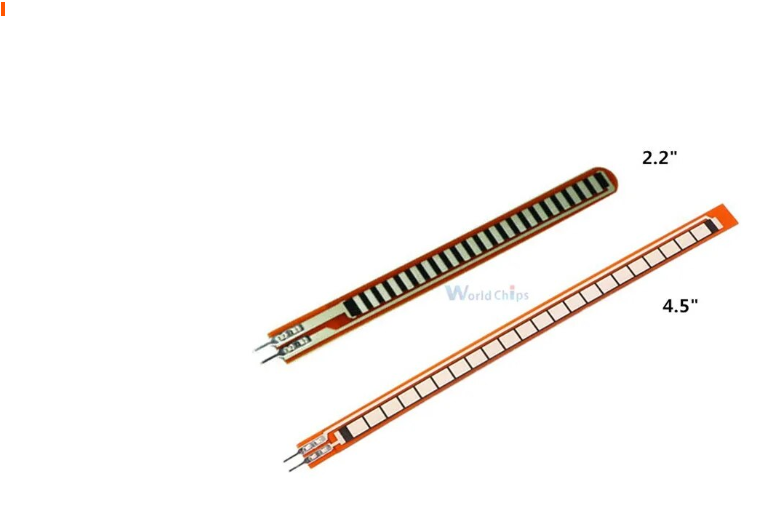
\includegraphics[width=9cm]{Images/Theoretical basis/flex sensor.png}
\caption{Flex sensor}
\end{figure}

\subsubsubsection{Nguyên lý hoạt động}

\begin{enumerate}[-]
    \item Mực dẫn trên cảm biến chính là một loại trở kháng. 
    \begin{itemize}
        \item Khi cảm biến thẳng, trở kháng này khoảng 25k.
        \item Khi cảm biến được uốn cong, lớp mực dẫn bị căng, dẫn đến giảm diện tích tiết diện (hãy tưởng tượng như việc căng một sợi dây cao su) và tăng trở kháng. Ở góc uốn cong 90°, trở kháng này khoảng 100K.
        \item Khi cảm biến được thẳng lại, trở kháng trở về giá trị ban đầu.
    \end{itemize}
    \item  Bằng cách đo trở kháng, ta có thể xác định được mức độ uốn cong của cảm biến.
\end{enumerate}

\begin{figure}[H]
    \centering
    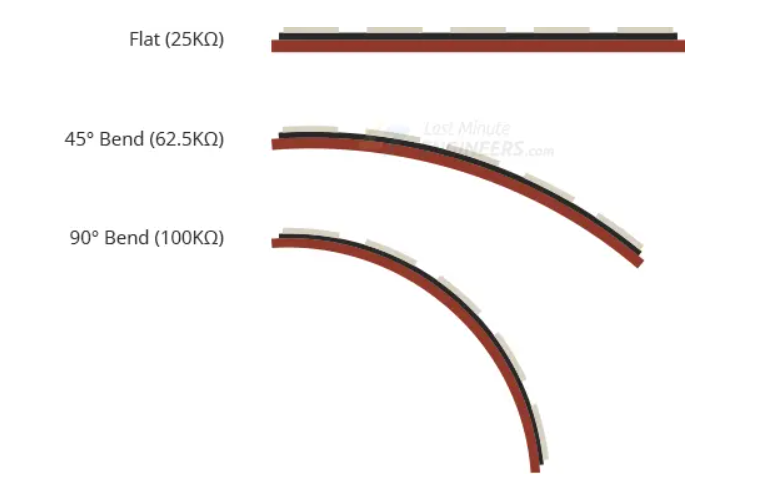
\includegraphics[width=11cm]{Images/Theoretical basis/flex sensor 1.png}
\caption{Hình dạng uốn cong của flex sensor}
\end{figure}

\subsubsubsection{Đọc giá trị}

\indent Cách đơn giản nhất để đọc cảm biến uốn cong (Flex Sensor) là kết hợp với một trở kháng tĩnh để tạo thành một bộ chia điện áp, từ đó tạo ra một điện áp biến đổi có thể đọc được bởi bộ chuyển đổi tương tự sang số của vi điều khiển.

\begin{figure}[H]
    \centering
    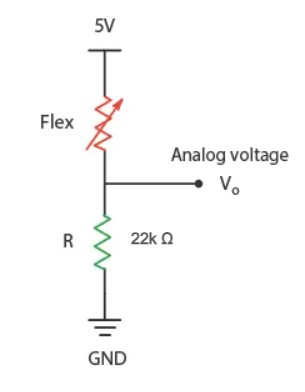
\includegraphics[width=5cm]{Images/Theoretical basis/flex sensor 2.jpg}
\caption{Sơ đồ nối dây của flex sensor}
\end{figure}

\indent Lưu ý rằng điện áp đầu ra mà bạn đo là mức giảm điện áp qua trở kháng kéo xuống, không phải là giảm điện áp qua cảm biến uốn cong (Flex Sensor).

\indent Chúng ta có thể sử dụng công thức sau để tính toán điện áp đầu ra (Vo).
\[ V_0 = \frac{V_{cc} \cdot R}{R + R_{\text{flex}}} \]

\indent Trong trường hợp này, điện áp đầu ra giảm khi bán kính uốn cong tăng lên.


\subsubsection{Arduino Nano}

\subsubsubsection{Giới thiệu chung về Arduino}

\indent Arduino một nền tảng vi mạch thiết kế mở phần cứng (Open-source hardware) và phần mềm (Open -source software). Phần cứng Arduino là những bộ vi điều khiển bo mạch đơn (Single-board microcontroller) được khởi động vào năm 2005 như là một dự án dành cho sinh viên tại Interaction Design Institude Ivrea tại thị trấn Ivrea ở Ý, nhằm xây dựng các ứng dụng tương tác với nhau hoặc với môi trường được thuận lợi hơn.

\indent Hiện nay Arduino được biết đến rất rộng rãi, từ học sinh trung học, đến sinh viên và người đi làm. Những dự án nhỏ và lớn được thực hiện một cách rất nhanh, các mã nguồn mở được chia sẻ nhiều trên diễn dàn trong nước và nước ngoài. Giúp ích rất nhiều cho những bạn theo đam mê nghiên cứu chế tạo những sản phẩm có ích cho xã hội. Trong những năm qua, Arduino là bộ não cho hàng ngàn dự án điện tử lớn nhỏ, từ những sản phẩm ra đời ứng dụng đơn giản trong cuộc sống đến những dự án khoa học phức tạp.

\indent Hiện nay trên thị trường có rất nhiều phiên bản Arduino như Arduino Uno R3, Arduino Uno R3 CH340, Arduino Mega2560, Arduino Nano, Arduino Pro Mino, Arduino Lenadro, Arduino Industrial.... Trong dự án lần này nhóm sẽ sử dụng board Arduino Nano Atmega328p vì đây là loại Arduino nhỏ gọn, giá thành hợp lí và đáp ứng đủ các yêu cầu của dự án.

\subsubsubsection{Đặc điểm kĩ thuật của Board Arduino Nano}

\begin{figure}[H]
    \centering
    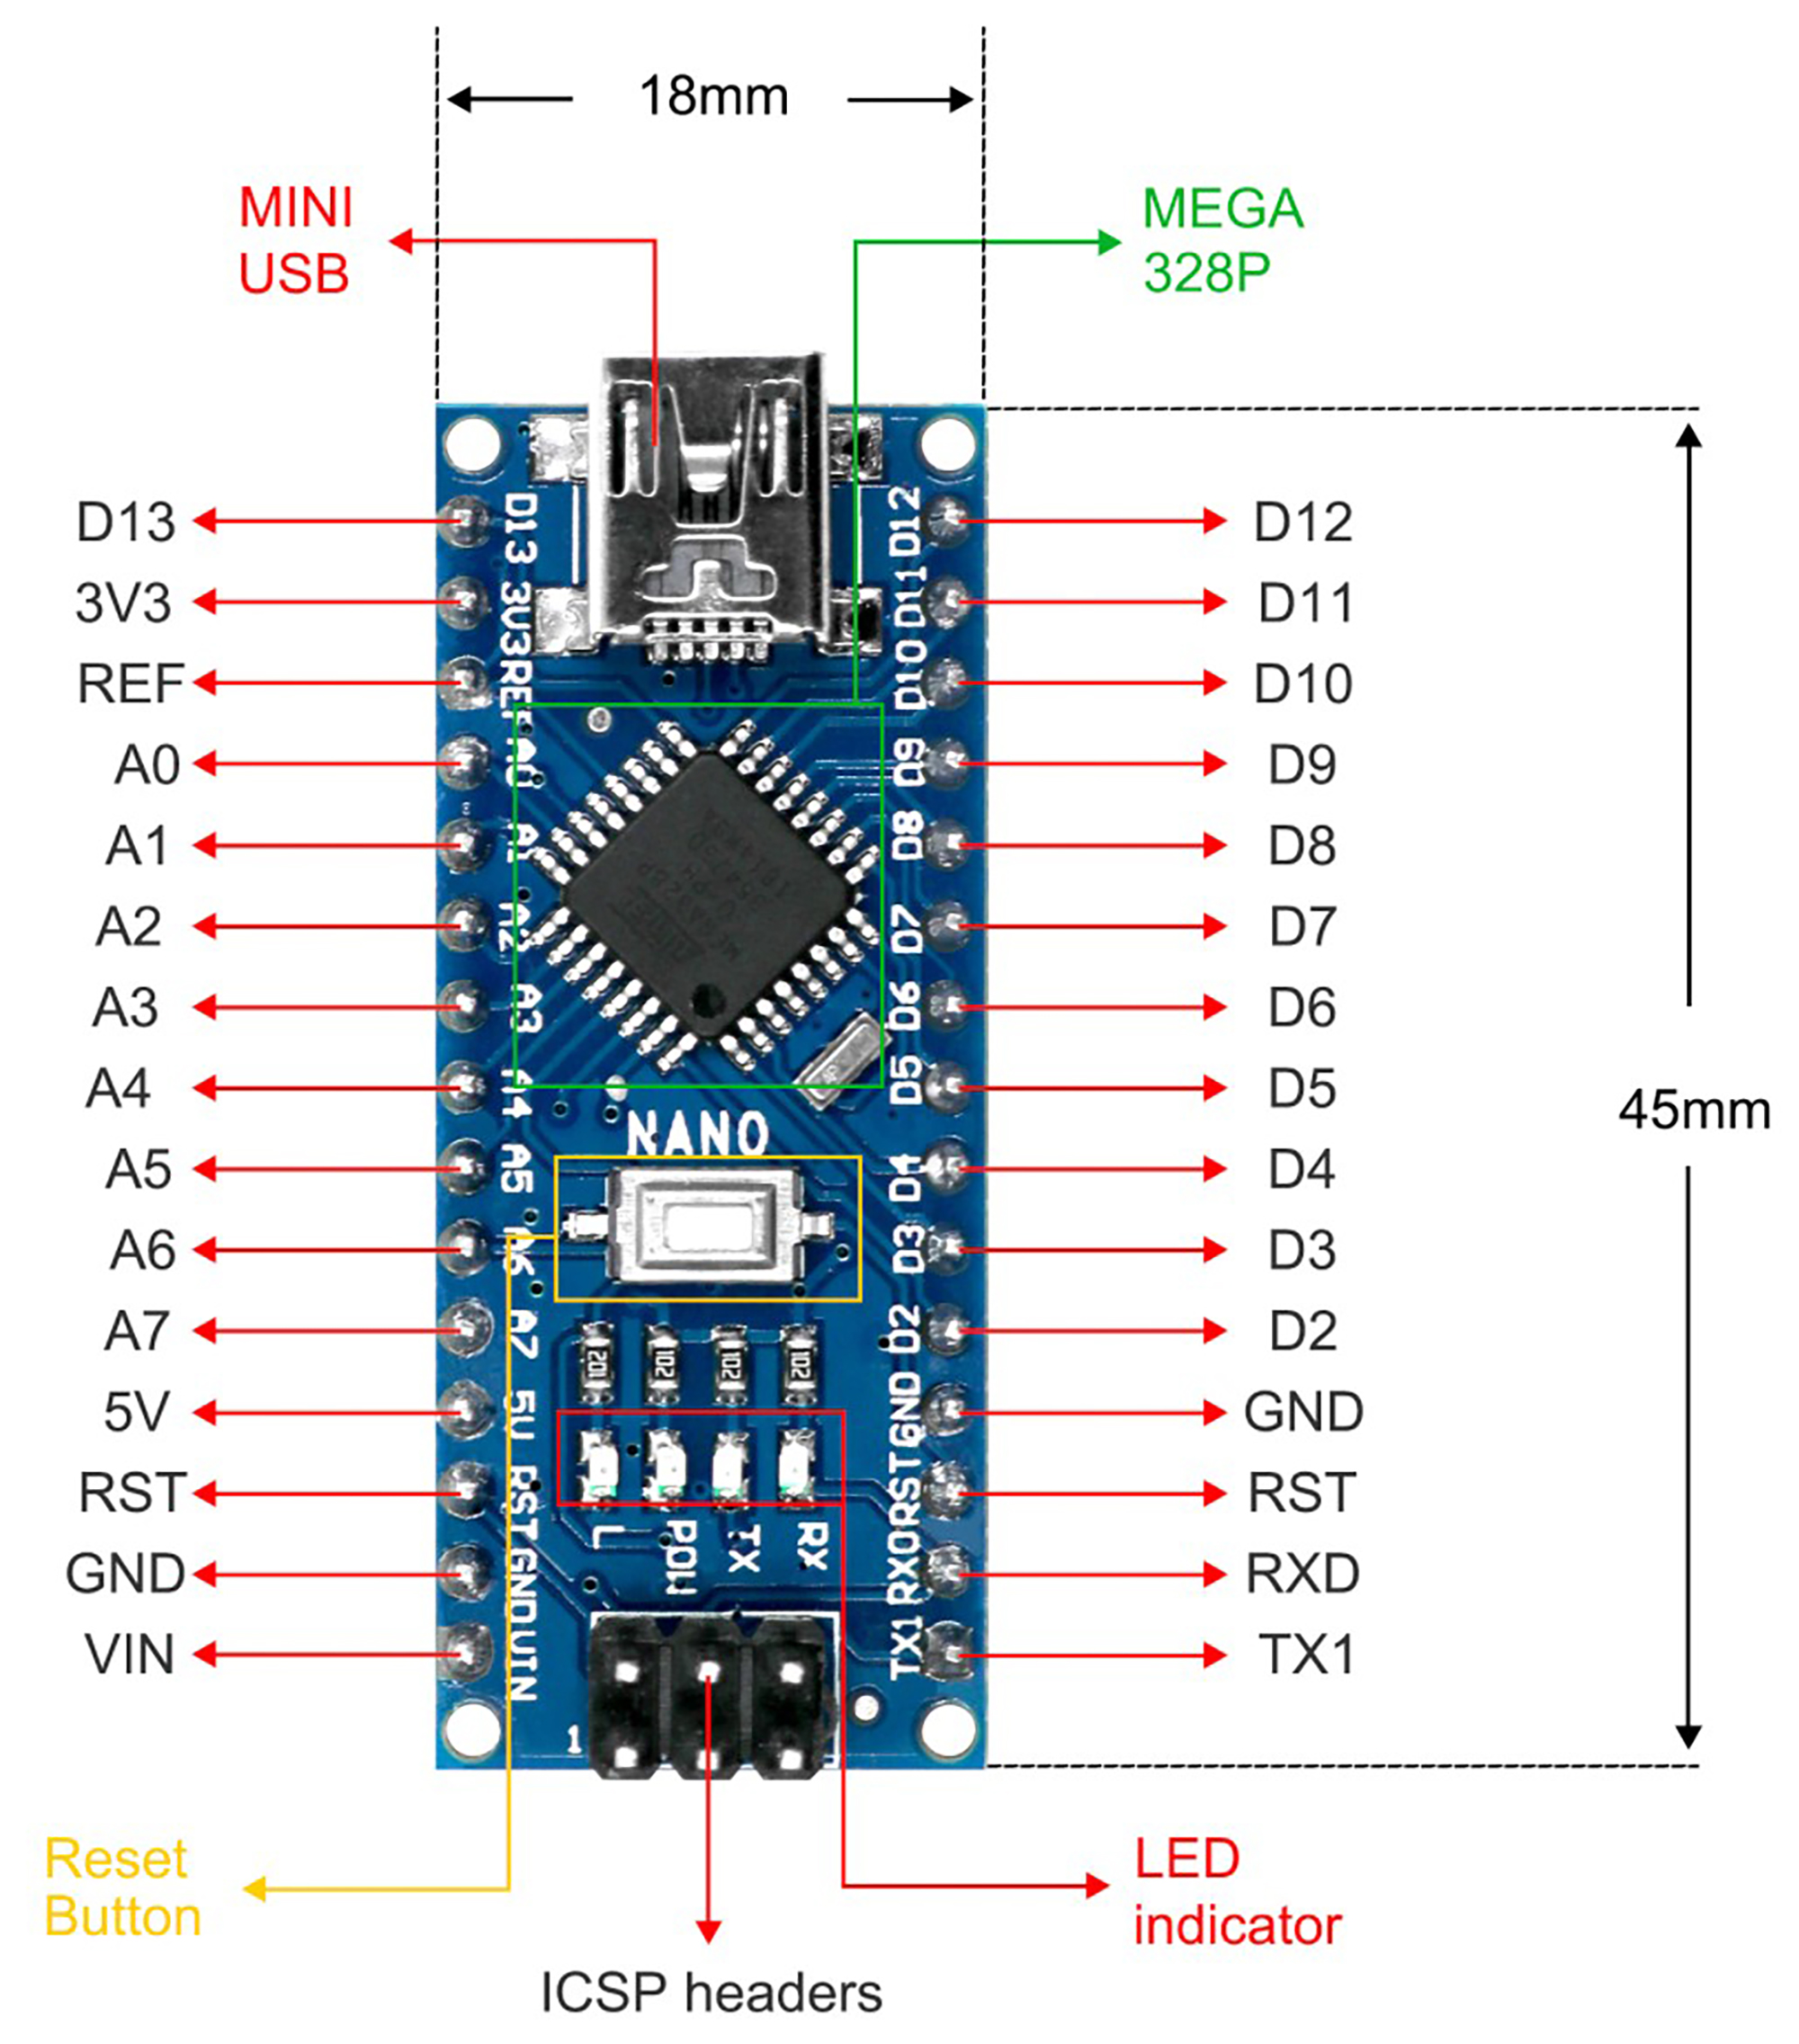
\includegraphics[width=8cm]{Images/Theoretical basis/arduino nano.jpg}
\caption{Arduino Nano}
\end{figure}

\begin{figure}[H]
    \centering
    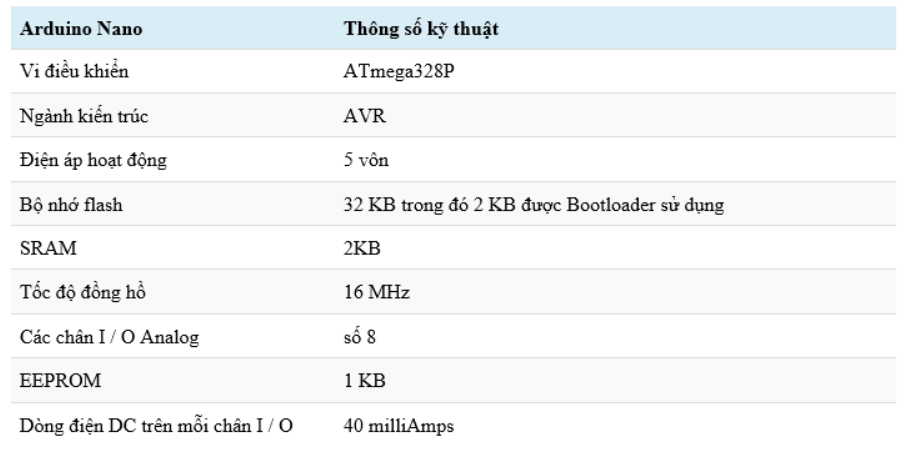
\includegraphics[width=13cm]{Images/Theoretical basis/arduino nano datasheet.png}
\caption{Thông số của Arduino Nano}
\end{figure}

\begin{enumerate}[-]
    \item Chân năng lượng:
    \begin{itemize}
        \item Vin (Nguồn vào): Chân này được sử dụng để cung cấp nguồn từ nguồn ngoại vi. Thường là từ 7V đến 12V.
        \item 5V (Nguồn 5V): Nguồn cung cấp 5V, thích hợp để cấp nguồn cho các module và cảm biến.
        \item 3.3V (Nguồn 3.3V): Nguồn cung cấp 3.3V, thích hợp cho các module hoạt động ở mức điện áp thấp.
        \item GND (Đất): Chân đất (Ground) chung cho hệ thống.
    \end{itemize}
    \item  Chân đầu vào/đầu ra Digital:
    \begin{itemize}
        \item D0 - D13: Chân I/O số từ 0 đến 13, dùng cho đầu vào và đầu ra số.
    \end{itemize}
    \item  Chân đầu vào Analog:
    \begin{itemize}
        \item A0 - A5: Chân đầu vào analog từ A0 đến A5.
    \end{itemize}
    \item  Chân giao tiếp Serial:
    \begin{itemize}
        \item TX (Transmit): Chân truyền dữ liệu, được sử dụng để truyền dữ liệu.
        \item RX (Receive): Chân nhận dữ liệu, được sử dụng để nhận dữ liệu.
    \end{itemize}
    \item  Chân giao tiếp I2C:
    \begin{itemize}
        \item A4 (SDA): Chân dữ liệu I2C.
        \item A5 (SCL): Chân xung đồng hồ I2C.
    \end{itemize}
    \item  Chân giao tiếp SPI:
    \begin{itemize}
        \item D10 (SS): Chân lựa chọn thiết bị SPI (Slave Select).
        \item D11 (MOSI): Chân dữ liệu SPI.
        \item D12 (MISO): Chân dữ liệu đầu ra SPI.
        \item D13 (SCK): Chân xung đồng hồ SPI.
    \end{itemize}
    \item  Chân Reset:
    \begin{itemize}
        \item RESET: Chân reset, được sử dụng để đặt lại vi xử lý.
    \end{itemize}
\end{enumerate}


\subsubsubsection{Ưu và nhược điểm của Arduino Nano}

\begin{enumerate}[-]
    \item Ưu điểm
    \begin{itemize}
        \item Arduino Nano có kích thước nhỏ, giúp tiết kiệm không gian và thuận tiện cho các ứng dụng có hạn về không gian.
        \item Arduino Nano có thể dễ dàng được lập trình và sử dụng giống như các board Arduino khác, với môi trường phần mềm Arduino IDE hỗ trợ.
        \item Arduino Nano thường có giá thành phải chăng, là lựa chọn phổ biến cho các dự án DIY và giáo dục.
        \item Arduino Nano có đầy đủ cổng kết nối bao gồm cả cổng USB, cổng nạp chương trình, và các chân GPIO để kết nối với các module và cảm biến khác.
    \end{itemize}
    \item  Nhược điểm
    \begin{itemize}
        \item ATmega328P có dung lượng bộ nhớ và tốc độ xử lý hạn chế so với một số vi điều khiển mạnh mẽ hơn, điều này có thể gây ra hạn chế trong việc xử lý các ứng dụng phức tạp.
        \item Arduino Nano có ít chân GPIO so với một số board Arduino khác, điều này có thể là một hạn chế cho các dự án yêu cầu nhiều chân GPIO.
        \item Vì kích thước nhỏ, có thể gặp khó khăn khi muốn mở rộng hoặc thay đổi các thành phần ngoại vi trên board.
        \item Với tốc độ xử lý và bộ nhớ có hạn, Arduino Nano có thể gặp khó khăn khi xử lý dữ liệu liên tục hoặc trong các ứng dụng đòi hỏi hiệu suất cao.
    \end{itemize}
\end{enumerate}